\chapter*[Introdução]{Introdução}
\addcontentsline{toc}{chapter}{Introdução}

O conceito de computação em nuvem está difundido como um novo paradigma para o desenvolvimento de sistemas, esse paradigma propõe a execução e o armazenamento através da internet sem a necessidade de programas no sistema local.

Uma das abordagens adotadas pela programação em nuvem é o Infrastructure as a service ou Infraestrutura como um serviço (IaaS), essa designação é feita para  definir um serviço executado na nuvem, que é feito através de máquinas virtuais que rodam nos clusters das empresas que disponibilizam esse serviço.

Um dos problema enfrentado por essas empresas é impacto financeiro e ambiental por deixar as máquinas ligadas, já que o custo elétrico delas pode se mostrar elevados pela grande quantidade de clusters ligados.

Nessa perspectiva uma das grandes áreas de busca dessas empresas é a consolidação de máquinas virtuais onde essa visa a minimização de máquinas ligadas, para isso várias limitações físicas devem ser levados em consideração como a quantidade de memória ram, processamento, barramento da internet, dentre outras que se apresentam em determinados contextos.

O objeto de estudo desse trabalho tende a se inclinar para o estudo dos recursos de processamento e ram e de conflitos entre maquinas virtuais, pois esses consolidam os problemas mais pertinentes na consolidação de maquinas virtuais.


\chapter{Problemática}

Para abranger a problemática envolvida na consolidação de maquinas virtuais deve se levar em conta os limites físicos e as regras estabelecidas no contexto das empresas abordando soluções que não penalizem a qualidade do serviço.

Para alcançar a consolidação de maquinas virtuais foi feita a analise do problema em duas parte uma visando a melhor alocação dos recursos físicos e outra corrigindo conflitos que essa alocação possa acarretar. 

\section{Recursos Físicos}

O problema da má gestão dos recursos físicos é um problema encontrado em grande partes da empresas, e como vantagem competitiva a optimização desses recursos pode alavancar em uma possível disputa empresarial.

No caso das empresas que prestam infraestrutura como um serviço, um dos objetos de maior desperdício será o processamento e a memoria de seus equipamentos, ja que uma alocação mal feita gerara espaços produz irar espaços vazios que poderiam ser utilizados para prover mais serviços.

Com a tecnologia atual dos computadores a má alocação em vista do consumo de energia foi minimizadas, fazendo com que uma maquina lotada e uma vazia gastem uma quantidade similar de energia, porem mesmo com essas melhorias, uma maquina inativa sempre consumira menos energia que uma ligada, portanto o problema da optimização persiste porem com o intuito de atribuir o máximo de serviço a menor quantidade de maquinas, para que assim haja uma economia inativando maquinas desnecessárias.

\section{Afinidade Entre Aplicações}

O problema de afinidade entre aplicações é um problema que afeta diretamente a solução de gerenciar os recursos físicos, esse problema consiste em aplicações que disputam algum recurso da maquina física, o que acarreta danos para aplicação de velocidade ou ate mesmo de indisponibilidade.

No caso do escopo do tópico 1.1 o problema se intensifica pois uma solução seria colocar o máximo numero de maquinas virtuais em menos recurso físicos ativos, porem isso aumenta a probabilidade que ocorra uma distribuição em que maquinas disputem os recursos.

\section{Conclusão}

Para que a consolidação das maquinas virtuais seja efetivada deve se considerar os dois principais problemas relatados, pois a solução baseada só em uma delas acarretaria em uma solução que prejudicaria a qualidade do serviços, o que não mostraria uma solução de viés satisfatória para a industria.
 
\chapter{Background}

Essa sessão é destinado ao levantamento teórico da solução proposta para o problema.

\section{Logica Proposicional}

A logica proposicional é um sistema formal destinado para a representação de proposições e sentenças declarativas, que podem possir valores verdadeiros ou falsos.

Uma logica proposicional possui regras estabelecidas para sua formulação onde é utilizado conectivos lógicos para seu desenvolvimento esses conectivos permitidos são $\land$ (e), $\lor$ (ou), $\lnot$ (negação), $\Rightarrow$ (se...então), $\iff$ (se e somente se). Através desses podemos construir sentenças compostas que são elaboradas através da junção de sentenças com conectores dando assim a possibilidade da representação de expressões logicas mais complexas.


\section{SAT}

A Satisfatibilidade Booleana ou SAT é um problema da classe dos NP-completos que dado uma expressão lógica com variáveis booleanas ele tenta determinar um o conjunto de variáveis que ao serem verdadeiras o valor da expressão também é verdadeiro.

Nesses quesitos quando a formulação é dita como satisfeita é quando ocorre que o conjunto da formulação é dado como verdadeiro, e não satisfeita quando é falso. 
 


Exemplo:
 
Dado as variáveis x1, x2 na expressão lógica $y = x1 \land x2$

\begin{center}
\begin{tabular}{ |c|c|c|c| } 
\hline
x1 & x2 & y & tipo\\
\hline
0 & 0  & 0 & solução não satisfeita \\ 
0 & 1 & 0  & solução não satisfeita \\ 
1 & 0 & 0  & solução não satisfeita \\
1 & 1 & 1  & solução satisfeita \\
\hline
\end{tabular}
\end{center}

\section{Pseudo Boolean}

As funções pseudo-booleanas tem intuito de realizar o mapeamento de valores booleanos para números reais, isso ocorre através do uso de variáveis booleanas junto a restrições de desigualdade linear com coeficientes inteiros que agem como um peso nas variáveis booleanas.
	
A vantagem do uso das funções pseudo booleanas esta na facilidade de abstração de problemas através das restriçoes pseudo booleanas, e por sua proximidade com SAT pode ser resolvida polinomialmente com o uso de SAT solvers.  

\chapter[Trabalhos Correlatos]{Trabalhos Correlatos}

\section{Introdução}

Esse capitulo visa dissecar e compreender os trabalhos que servem como base para o desenvolvimento desse projeto.

Pela a proposta de resolução do problema se basear em técnicas pseudo-booleanas e optimização por restrições, o capitulo trabalhara em cima dos seguintes estudos:

\begin{itemize}
    \item On Modelling Virtual Machine Consolidation to
    Pseudo-Boolean Constraints \cite{bruno2012}
    \item PBFVMC: A New Pseudo-Boolean Formulation to Virtual-Machine Consolidation \cite{bruno2013}
    \item Um método de pré-processamento de fórmulas sat e pseudo-boolean baseado em tecnicas de programação linear inteira mista. \cite{bruno2015}
    \item Afinidades de tipos de aplicações em nuvens computacionais.\cite{fabio2014}
\end{itemize}

Os trabalhos citados a cima são divididos em duas formulações que visão encontrar uma decisão satisfatória para o problema em menor tempo hábil. Por esse motivo a estrutura desse capitulo comtemplara uma primeira formulação vigente ao trabalho \cite{bruno2012} e apos isso sera analizado a evolução da formulação que se encontra no trabalho \cite{bruno2013}. 


\section{Primeira Formulação Pseudo Booleana}

Como explicado no topico 3.3 sobre logica pseudo booleana, para representar um problema através dessa logica é necessário abstrair o problema em variáveis booleanas e disjunções de grandeza.

Na solução definida no artigo \cite{bruno2012} e definido seis conjuntos de restrições para minimizar o uso de maquinas ligadas, a obtenção dessas formulas foram feita através da abstração do problema e essas são:
 
 \subsection{Formula Objetivo}
 
 A primeira formula definida diz respeito ao objetivo do problema que é minimizar o numero de maquinas físicas ligadas e matematicamente é expressa por: 
 
 $$[1] \qquad min: \sum_{i=1}^{n} hw_{i}$$	


 \subsection{Recurso Necessário Disponível}
 
 A segunda é terceira formula proposta diz respeito a verificação se a quantidade de ram e processamento das maquinas somadas se equivalem ao somatório da quantidade respectiva das maquinas virtuais. 

 $$[2] \qquad \sum_{i=1}^{n} RAM_{hwi} . hw_{i}^{ram} \geq \sum_{j=1}^{n} RAM_{vmj} \cdot vm_{j}^{ram} $$	


 $$[3] \qquad  \sum_{i=1}^{n} PROC_{hwi} . hw_{i}^{proc} \geq \sum_{j=1}^{n} PROC_{vmj} \cdot vm_{j}^{proc} $$	
 
 
 \subsection{Limitar Recurso por Hardware}

As duas clausulas definidas aqui diz respeito a limitação do uso do hardware pela maquinas virtuais, ela faz com que um hardware não etoure sua capacidade de alocar maquinas virtuais nele.  
 
 $$[4] \qquad \forall hw_{i}^{ram} \in hw_{n}^{ram} (\sum_{j = 1}^{k}  RAM_{vmj}
\cdot vm^{ram \cdot hwi}_{j} \leq RAM_{hwi})  $$

 $$ [5] \qquad  \forall hw_{i}^{proc} \in hw_{n}^{proc} (\sum_{j = 1}^{k}  PROC_{vmj}
\cdot vm^{proc \cdot hwi}_{j} \leq PROC_{hwi})  $$


\subsection{Uma Maquina Virtual por Harware}

A ultima restrição proposta é elaborada com o intuito de restringir o uso de uma Maquina virtual por hardware.

$$[6] \qquad \forall vm_{i} \in vm_{K} (\sum_{j = 1}^{n} vm_i^{proc \cdot hwj} \cdot vm_{i}^{ram \cdot hwj} \cdot hw_{j}^{proc} \cdot hw_{j}^{ram} = 1) $$
  
\subsection{Exemplo}

Nessa sub-seção sera mostrado um exemplo da construção das formulas da primeira formulação dado um conjunto de hardwares e maquinas virtuais.

Sendo estes:

\begin{table}[!htb]
    \caption{hardware e maquinas virtuais}
    \begin{minipage}{.5\linewidth}
      \caption{Hardware}
      \centering
        \begin{tabular}{ |c|c|c| } 
            \hline
            Nome & Ram & Processamento\\
            \hline
             hw1 & 100 & 20  \\ 
             hw2 & 30 & 10  \\ 

            \hline
        \end{tabular}
    \end{minipage}%
    \begin{minipage}{.5\linewidth}
      \centering
        \caption{Maquinas Virtuais}
        \begin{tabular}{ |c|c|c| } 
            \hline
            Nome & Ram & Processamento\\
            \hline
            vm1 & 50  & 5  \\ 
            vm2  & 30 & 20  \\ 
            vm3 & 10 & 5   \\
            \hline
        \end{tabular}
    \end{minipage} 
\end{table}

A partir desses dados geramos as restrições citadas anteriormente, onde para formula [1] temos:

    $$min: \quad hw1 + hw2 $$

para [2] e [3]:

    $$ 100 \cdot hw_1^{ram} + 30 \cdot hw_2^{ram} \geq 90$$

    $$ 20 \cdot hw_1^{proc} + 10 \cdot hw_2^{proc}  \geq 30$$
    

formula [4]:

$$ 50 \cdot vm_1^{ram \cdot hw1} + 30 \cdot vm_2^{ram \cdot hw1} + 10 \cdot vm_3^{ram \cdot hw1}\leq 100$$


$$ 50 \cdot vm_1^{ram \cdot hw2} + 30 \cdot vm_2^{ram \cdot hw2} + 10 \cdot vm_3^{ram \cdot hw2}\leq 30$$

formula [5]:

$$ 5 \cdot vm_1^{proc \cdot hw1} + 20 \cdot vm_2^{proc \cdot hw1} + 5 \cdot vm_3^{proc \cdot hw1}\leq 20$$


$$ 5 \cdot vm_1^{proc \cdot hw2} + 20 \cdot vm_2^{proc \cdot hw2} + 5 \cdot vm_3^{proc \cdot hw2}\leq 10$$

Formula [6]:


$$vm_1^{proc \cdot hw1} \cdot vm_{1}^{ram \cdot hw1} \cdot hw_{1}^{proc} \cdot hw_{1}^{ram} + vm_1^{proc \cdot hw2} \cdot vm_{1}^{ram \cdot hw2} \cdot hw_{2}^{proc} \cdot hw_{2}^{ram} = 1 $$


$$vm_2^{proc \cdot hw1} \cdot vm_{2}^{ram \cdot hw1} \cdot hw_{1}^{proc} \cdot hw_{1}^{ram} + vm_2^{proc \cdot hw2} \cdot vm_{2}^{ram \cdot hw2} \cdot hw_{2}^{proc} \cdot hw_{2}^{ram} = 1 $$


$$vm_3^{proc \cdot hw1} \cdot vm_{3}^{ram \cdot hw1} \cdot hw_{1}^{proc} \cdot hw_{1}^{ram} + vm_3^{proc \cdot hw2} \cdot vm_{3}^{ram \cdot hw2} \cdot hw_{2}^{proc} \cdot hw_{2}^{ram} = 1 $$

\section{Segunda Formulação Pseudo Booleana}

\subsection{Formula Objetivo}
 
 Como na abordagem da primeira formulação o principal objetivo é reduzir as maquinas virtuais ligada, e com isso a formula se manteve a mesma.

 $$[1] \qquad min: \sum_{i=1}^{n} hw_{i}$$	

\subsection{Acomodar recursos em hardwares ligados}

As duas formulas a seguir redtrigem que o somatorio dos recursos dos hardwares ligados acomodem os recursos utilizados pela maquinas virtuais.

$$[1] \qquad \sum_{i=1}^{n} Ram_{hwi} \cdot hw_{i} \geq \sum_{j=1}^{k} Ram_{vmj} $$

$$[1] \qquad \sum_{i=1}^{n} Proc_{hwi} \cdot hw_{i} \geq \sum_{j=1}^{k} Proc_{vmj} $$

\subsection{Limites superiores}

As restriçoes a seguir di respeito ao quanto de recurso as maquinas podem prover as maquinas virtuais


$$[1] \qquad \forall i \in 1..n (\sum_{j=1}^{k} (Ram_{vmj} \cdot \lnot{vm_{j}^{hwi}}) + Rhw_{i} \cdot hw_i \geq \sum_{j=1}^{k} Ram_{vmj})$$

$$[1] \qquad \forall i \in 1..n (\sum_{j=1}^{k} (Proc_{vmj} \cdot \lnot{vm_{j}^{hwi}}) + Rhw_{i} \cdot hw_i \geq \sum_{j=1}^{k} Proc_{vmj})$$

\subsection{Alocação Obrigatoria}

Essa restrição define que cada maquina virtual deve esta alocada a um hardware.

$$[1] \qquad \forall i \in 1..n  \sum_{j=1}^{k} (vm_j^{hwi} \geq 1)$$

\subsection{Alocação unica}

E por fima ultima restrição garnte que uma maquina virtual possui alocação em apenas em um hardware, não podendo dividir os recursos da vm para distruibuir.

$$[1] \qquad \forall \quad i  \in 1..K (\sum_{i=1}^{N} \lnot{vm_j^{hwi}} \geq N - 1)$$

\subsection{Exemplo}

Nessa seção será mostrado a construção das formulas utilizando a segunda formulação, sera atribuído os mesmos valores do exemplo 3.2.5.

[1]

$$min: \quad hw1 + hw2 $$

[2] e [3]

$$100 \cdot hw_1 + 30 \cdot hw_2 \geq 90$$ 


$$20 \cdot hw_1 + 10 \cdot hw_2 \geq 30$$ 


[4] e [5]

$$ (50 \cdot \lnot{vm_1^{hw1}}) + (30  \cdot \lnot{vm_2^{hw1}}) + (10  \cdot \lnot{vm_3^{hw1}}) + 100 \cdot hw_1 \geq 90 $$ 

$$ (50 \cdot \lnot{vm_1^{hw2}}) + (30  \cdot \lnot{vm_2^{hw2}}) + (10  \cdot \lnot{vm_3^{hw2}}) + 30 \cdot hw_2 \geq 90 $$ 


$$ (5 \cdot \lnot{vm_1^{hw1}}) + (20  \cdot \lnot{vm_2^{hw1}}) + (5  \cdot \lnot{vm_3^{hw1}}) + 30 \cdot hw_1 \geq 30 $$ 


$$ (5 \cdot \lnot{vm_1^{hw2}}) + (20  \cdot \lnot{vm_2^{hw2}}) + (5  \cdot \lnot{vm_3^{hw2}}) + 30 \cdot hw_2 \geq 30 $$

[6]

$$ vm_1^{hw1} + vm_2^{hw1} + vm_3^{hw1} \geq 1 $$


$$ vm_1^{hw2} + vm_2^{hw2} + vm_3^{hw2} \geq 1 $$

[7]

$$(\lnot{vm^{hwi}_j} + \lnot{vm_k^{hwi}})$$\

\section{Afinidade de aplicações}

Essa seção visa trabalhar com as classes de aplicações e suas afinidades, seguindo o estudo afinidades de tipos de aplicações em nuvens computacionais \cite{fabio2014}.

O estudo baseia se em classes de aplicações que podem ser rodadas nas maquinas virtuais chamadas de classes dwarfs essas sendo divididas em treze categorias sendo essas:

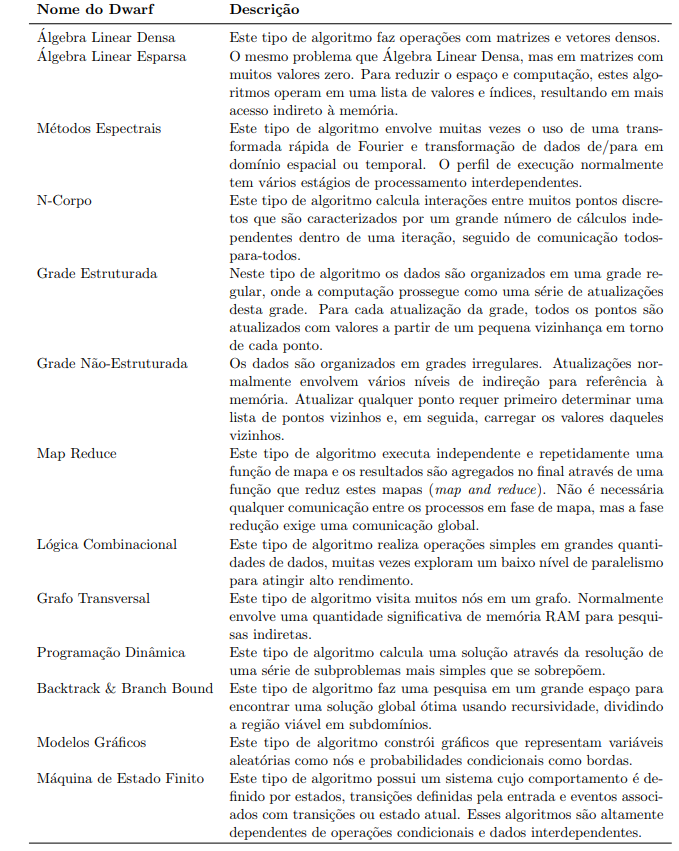
\includegraphics[width=0.9\textwidth]{tabela_dwarf.png}

Porem para o estudo foram realizados os testes apenas com os dwarfs de grafo transversal, grade estruturada e matriz densa, pois esses contemplam a maiorias das aplicações que necessitam de hospedagem.

Para o desenvolvimento do estudo foi utilizado as bibliotecas de programação paralela OpenCL e OpenMP junto do pacote de brenchmark rodinia, que possuem módulos característicos dos tipos de dwarfs citados.


\chapter[Proposta]{Proposta}

A proposta levantada nessa etapa e que sera executada no trabalho de conclusão de curso 2 é uma tercerira evolução da formulação pseudo booleana apresentada anteriormente de modo que a solução se enquadre ainda mais no problema real encontrado no gerenciamento da alocação de maquinas virtuais.

Na modelagem atual a formulação faz a optimização considerando apenas alocação das maquinas por quantidade de cpu e memoria ram, porem essa abordagem considerando apenas isso desconsidera uma possibilidade que ocorre no mundo real de concorrência entre maquinas virtuais.

Portanto é esperado que ao estender a formulação seja possível manter o padrão que a segunda formulação traz de minimizar os equipamentos ligados, porem evitando conflitos com aplicações com baixa afinidade.

Para a conclusão no projeto em sua totalidade é esperado que as seguintes perguntas sejam respondidas:

\begin{itemize}
    \item A solução tem aplicabilidade real ?
    \item Qual o custo do algorítimo ?
    \item Quais métricas devem ser consideradas para determinar se o tempo do algorítimo é viável ?
    \item O algorítimo possui um ponto onde deixa de compensar ?
    \item O algorítimo pode ser melhorado ? 
    \item As restrições da segunda formulação pode ser aprimoradas ?
    \item É necessário acrescentar novas restrições ou um pre-processamento dos dados resolve o problema ?  
\end{itemize}



\section{Etapas do Projeto}

\subsection{Estudo}
\subsection{Preparação dos dados}
\subsection{Ciclo de Formulação e testes}
\subsubsection{Avaliação e Comparativo}


\section[Cronograma]{Cronograma}
